\newpage
\section{Full-Text Search}
Commercial database management has long focused on structured data and the industry requirements have matched those of structured storage applications quite well.
The problem is that only a small part of the data stored is completely structured, while most of it is completely unstructured or only semi-structured, in the form of documents, emails, web pages, etc. \parencite[cf.][p. 7]{hamilton_microsoft_2001}\\
\subsection{Microsoft SQL Server Search Architecture}
\ac{SQL} Server uses the same access method and infrastructure for full-text search as other \ac{MS} products and the Index Service for file systems. This decision enables standardized semantics for full-text search of data in relational databases, web-hosted data, and data stored in the file system and mail systems. On \ac{SQL} servers, not only simple strings can be indexed, but also data structures, such as \ac{HTML} and \ac{XML}, and even complex documents, such as \ac{PDF}, Word, PowerPoint, Excel and other custom document formats. \parencite[cf.][p. 7]{hamilton_microsoft_2001}\\
The architecture can be divided into five modules, which interact with each other to perform a full-text search. (See Figure \ref{fig:sql_search_architecture})\\
The \textbf{content reader} scans indexed data stored in \ac{SQL} Server tables to assemble data and its associated metadata packets. These packets are then injected into the main search engine, which triggers the search engine filter daemon to consume the data.\\
Depending on the content, the \textbf{filter daemon} calls different filters, which parse the content and output so-called chunks of the processed text. A chunk is a related section with relevant information about this section like the language-id of the text. These chunks are output separately for any properties, which can be elements like the title, an author or other content-specific elements.
\begin{figure}[H]
    \caption{Architecture of MS SQL Server Full-Text Search}
    \label{fig:sql_search_architecture}
    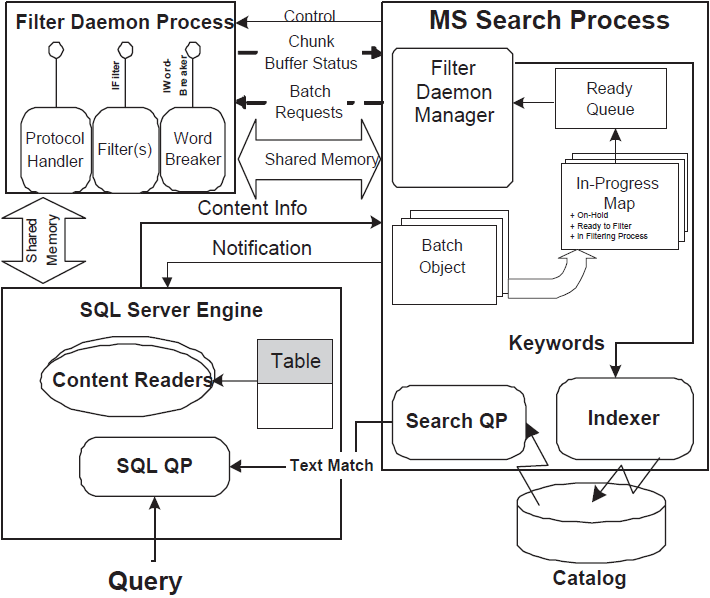
\includegraphics[width=0.9\textwidth]{sql_search_architecture.png}
    \\
    \cite[Source:][p. 8]{hamilton_microsoft_2001}
\end{figure}
\textbf{Word breakers} split the chunks into keywords and additionally provide alternative keywords and the corresponding position in the text. Word breakers can recognize human languages and on \ac{MS} \ac{SQL} Server several word breakers for different languages are installed by default. The generated keywords and metadata are passed on to the MS Search process, which processes the data with an indexer.\\
The \textbf{indexer} generates an inverted keyword list with a batch containing all keywords of one or more items. These indexes are compressed to use memory efficiently, this may lead to high costs for updates of these indexes. Therefore a stack of indexes is maintained. New documents first create their own small indexes, which are regularly merged into a larger index, which in turn is merged into the base index. This stack can be deeper than three, but the concept remains and allows a strongly compressed index without driving the update costs too high. If a keyword is searched, all indexes are accessed, so the depth should still be kept reasonable.\\
A \textbf{query processor} manages the insertion and merge operations and collects statistics on distribution and frequency for ranking purposes and query execution. \parencite[cf.][pp. 8-9]{hamilton_microsoft_2001}